\sect{Математические основы моделей отслеживания партитуры}{math}
%
Математический аппарат отслеживания партитуры удобно строить от
простого к сложному: первый кирпич~--- классический алгоритм
Dynamic Time Warping, второй~--- его каузальная модификация
On-line Time Warping, третий~--- скрытые марковские модели в
формулировке Рабинера~\cite{Rabiner1989} и их прикладная
адаптация для отслеживания партитуры, четвёртый~--- полу-марковские
расширения с явной длительностью состояний и гибридная
архитектура Конта~\cite{Cont2010}. Все обозначения соответствуют
принятой в литературе
нотации~\cite{Rabiner1989,Cont2010,Mueller2007}, и для
самостоятельности изложения каждая модель выводится из
предшествующей.
Отдельно (см.~\Secref{ssmm-df}) обсуждаются два метода~---
slotted symbolic Markov modeling и distribution fields,~---
оригинально развитые в смежной области астроинформатики и
потенциально применимые в нашей задаче.

\paragraph*{Запись партитуры на нотном стане.} Прежде чем
формализовать математику, полезно зафиксировать сам объект
изучения. Партитура~--- это упорядоченная последовательность
нот; каждой ноте соответствует пара (высота, длительность).
В дальнейшем для сквозного учебного примера используем мажорное
арпеджио из пяти нот:
$S_{\text{ex}} = (\text{C4, E4, G4, A4, C5})$,
с MIDI-кодами $(60, 64, 67, 69, 72)$ соответственно. Этот
пример выбран минимальным: пять нот достаточно, чтобы
проиллюстрировать все рекуррентные формулы, и одновременно
короток для пошагового численного разбора.

\par\addvspace{2pt}
{\centering
\refstepcounter{figure}\figlab{notes-example}%
% =====================================================================
% TikZ figure: 5-note example score on a treble staff (C4, E4, G4, A4, C5).
% Used as the running example throughout sections/04-math-foundations.tex.
% Pure black-and-white drawing without external glyphs.
% =====================================================================
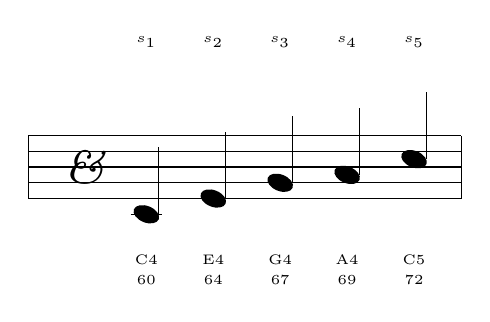
\begin{tikzpicture}[x=1mm,y=1mm,line width=0.4pt,font=\scriptsize]

  \def\stafflen{55}
  \def\noteh{1.4}
  % --- five horizontal lines of the treble staff ---
  \foreach \y in {0,2,4,6,8} \draw (0,\y) -- (\stafflen,\y);

  % --- bar lines ---
  \draw (0,0) -- (0,8);
  \draw (\stafflen,0) -- (\stafflen,8);

  % --- treble clef placeholder (simplified G-clef as text; not a real glyph) ---
  \node[anchor=west, scale=2.4] at (1.5, 4) {\textit{\&}};

  % --- note positions on the staff lines (treble clef):
  %   C4 = below the staff (1 ledger line below)
  %   E4 = bottom line          (y = 0)
  %   G4 = second line          (y = 2)
  %   A4 = second space         (y = 3)
  %   C5 = third space          (y = 5)
  % We place noteheads as filled ellipses; stems and labels below.
  \def\noteX{15} \def\noteSp{8.5}

  % helper: short ledger line for C4 below staff
  \draw (\noteX-2.0,-2) -- (\noteX+2.0,-2);

  \foreach \i/\xshift/\y/\name/\midi in {%
    1/0/-2/C4/60,
    2/1/0/E4/64,
    3/2/2/G4/67,
    4/3/3/A4/69,
    5/4/5/C5/72
  } {
    \pgfmathsetmacro{\xc}{\noteX + \xshift*\noteSp}
    % filled notehead (ellipse rotated)
    \begin{scope}[shift={(\xc,\y)},rotate=-22]
      \fill (0,0) ellipse (1.7 and 1.05);
    \end{scope}
    % stem upward
    \draw (\xc+1.6,\y) -- (\xc+1.6,\y+8.5);
    % label below
    \node[below=4mm,font=\tiny] at (\xc,-2) {\name};
    \node[below=6.5mm,font=\tiny] at (\xc,-2) {\midi};
  }

  % --- index labels above (i = 1..5) ---
  \foreach \i in {1,2,3,4,5} {
    \pgfmathsetmacro{\xc}{\noteX + (\i-1)*\noteSp}
    \node[above=10mm,font=\tiny] at (\xc,8) {$s_{\i}$};
  }

\end{tikzpicture}
\par
\vspace{2pt}
\footnotesize
\figurename~\thefigure. Сквозной учебный пример: пять нот
$(\text{C4, E4, G4, A4, C5})$ на нотном стане в скрипичном
ключе. На все последующие алгоритмы DTW, HMM и Forward будут
применяться именно к этому фрагменту.\par}
\addvspace{4pt}

\paragraph*{Dynamic Time Warping.} Прежде всего поясним, для
чего нужна эта конструкция. Допустим, у нас есть две
последовательности признаков, описывающих одно и то же
музыкальное событие, но идущих с разной скоростью: например,
эталонная синтезированная по партитуре аудиодорожка $A =
(a_1, \dots, a_I)$ длины $I$ кадров и реальная запись
исполнения $B = (b_1, \dots, b_J)$ длины $J$ кадров (как
правило $J \ne I$, потому что исполнитель играет с собственным
темпом). Задача~--- найти такое \textit{нелинейное} соответствие
между кадрами $A$ и $B$, при котором соотнесённые между собой
кадры были максимально похожи по своему содержанию.

Формально соответствие задаётся \textit{путём выравнивания}~---
последовательностью пар индексов $F = c(1), c(2), \dots, c(K)$,
где $c(k) = (i(k), j(k))$ означает «$i(k)$-й кадр $A$
сопоставлен с $j(k)$-м кадром $B$ на $k$-м шаге пути».
Допустимый путь обязан стартовать в левом нижнем углу матрицы
индексов и заканчиваться в правом верхнем
($c(1) = (1, 1)$, $c(K) = (I, J)$); ходить по этой матрице можно
только вправо, вверх или по диагонали (ровно на одну клетку),
что и обеспечивает условия монотонности
$i(k-1) \le i(k)$, $j(k-1) \le j(k)$ и непрерывность шага.

«Похожесть» двух кадров измеряется \textit{локальной стоимостью}
$d(i, j) = \|a_i - b_j\|$ (например, евклидовым расстоянием
между chroma-векторами); чем меньше $d(i, j)$, тем больше
сходство. Сложив локальные стоимости вдоль всего пути с
весами $w(k)$, получаем суммарную стоимость
$E(F) = \sum_{k=1}^K d(c(k))\,w(k)$. Веса $w(k) \ge 0$ нужны,
чтобы все три типа шага (вправо, вверх, по диагонали)
давали соразмерный вклад: например, в симметричной форме
Сакоэ-Чибы~\cite[уравн.~12]{SakoeChiba1978} диагональный шаг
получает вес~$2$, а горизонтальный и вертикальный~--- по~$1$
(подробное обсуждение разных весовых схем~---
в~\cite[\S~II-B]{SakoeChiba1978}).

Теперь содержательный вопрос: что значит «оптимальное»
выравнивание двух последовательностей? Если бы мы просто брали
путь с минимальной суммой $E(F)$, выгоднее всего было бы
двигаться кратчайшим путём (короткий путь даёт меньшее число
слагаемых даже при больших $d$). Чтобы устранить это
смещение, Сакоэ и Чиба нормируют сумму на сумму весов и
определяют \textit{нормализованное расстояние} как минимум
по всем допустимым путям:
\begin{equation}
D(A, B) \;=\; \min_{F}\;
\dfrac{\displaystyle\sum_{k=1}^{K} d(c(k))\,w(k)}
      {\displaystyle\sum_{k=1}^{K} w(k)}.
\eqlab{dtw-norm}
\end{equation}
Знаменатель~$\sum_k w(k) = N$~--- это, по сути, длина пути в
весовом смысле; для симметричной формы $N = I + J$, для
асимметричной $N = I$~\cite[уравн.~13--15]{SakoeChiba1978}.
Деление на $N$ делает $D(A, B)$ среднестрочной локальной
стоимостью на пути и убирает преимущество коротких путей.

Геометрически минимум в~\eqref{eq:dtw-norm} соответствует
поиску \textit{ломаной из нижнего левого угла в верхний
правый} в прямоугольной матрице $I \times J$, на каждой ячейке
которой лежит число $d(i, j)$, и эта ломаная должна давать
минимальную сумму чисел вдоль себя (с учётом весов). Прямой
перебор всех возможных путей экспоненциален по длине~$K$, но
существует элегантный приём~--- \textit{динамическое
программирование}: каждая частичная стоимость $g(i, j)$ на
ячейке $(i, j)$ зависит только от трёх соседних ячеек снизу и
слева, и поэтому матрицу $g$ можно заполнить за время
$O(IJ)$. Для практической реализации применяется рекурсивная
DP-формулировка~\cite[уравн.~16--18]{SakoeChiba1978}:
$g_1(c(1)) = d(c(1))\,w(1)$,
\begin{equation}
g_k(c(k)) = \min_{c(k-1)} \bigl[\,g_{k-1}(c(k-1)) +
                                 d(c(k))\,w(k)\,\bigr],
\eqlab{dtw-dp}
\end{equation}
$D(A,B) = g_K(c(K))/N$, где $N=\sum_k w(k)$. Для симметричных весов
$w(k) = (i(k)-i(k-1)) + (j(k)-j(k-1))$ и нулевого ограничения
наклона рекурсия принимает компактный вид
\begin{equation}
g(i,j) = \min\!\begin{cases}
g(i-1,j-1) + 2d(i,j),\\
g(i-1,j) + d(i,j),\\
g(i,j-1) + d(i,j),
\end{cases}
\eqlab{dtw-symmetric}
\end{equation}
с инициализацией $g(1,1)=2d(1,1)$ и итоговым $D(A,B)=g(I,J)/(I+J)$.
Для уменьшения вычислительной сложности с $O(NM)$ до $O(NR)$
применяется \textit{полоса Сакоэ-Чибы} $|i(k)-j(k)|\le R$~\cite[уравн.~8]{SakoeChiba1978}.

В контексте отслеживания партитуры~\cite{Mueller2007,Arzt2016}
последовательность $A$ обычно соответствует синтезированной по
партитуре аудиодорожке (или последовательности нот), $B$~---
живому исполнению; локальная стоимость $d(i,j)$ строится по
chroma-векторам, спектральным признакам или, как в современной
работе~\cite{ArztLattner2018}, по обучаемым транспозиционно-
инвариантным эмбеддингам.

\paragraph*{Пример заполнения матрицы DTW.} Пусть партитура~---
наш сквозной пример $S_{\text{ex}} = (60, 64, 67, 69, 72)$, а
исполнение содержит шесть событий с реализованными высотами
$P_{\text{ex}} = (60, 64, 67, 67, 69, 72)$ (третья нота сыграна
дважды~--- типичная исполнительская «зацепка»). В качестве
локальной стоимости используем
$d(i,j) = |\text{midi}(s_i) - q_j|$ в полутонах. Прямой расчёт
матрицы $g(i,j)$ по~\Eqref{dtw-symmetric} даёт нижеследующую
таблицу (показаны только значения внутри полосы Сакоэ-Чибы
$|i-j|\le 2$, остальные ячейки помечены прочерком):

\par\addvspace{2pt}
{\centering
\footnotesize
\begin{tabular}{c|cccccc}
\toprule
$i\backslash j$ & 1 & 2 & 3 & 4 & 5 & 6 \\
\midrule
1 (C4=60) & \textbf{0} & 4  & ---& ---& ---& ---\\
2 (E4=64) & 4 & \textbf{0}  & 3  & 3  & ---& ---\\
3 (G4=67) & ---& 3  & \textbf{0}  & \textbf{0}  & 2 & ---\\
4 (A4=69) & ---& ---& 2  & 2  & \textbf{0}  & 3 \\
5 (C5=72) & ---& ---& ---& 5 & 3 & \textbf{0} \\
\bottomrule
\end{tabular}\par
\vspace{2pt}}
\addvspace{4pt}

Жирным показан оптимальный путь $W = (1,1)\to(2,2)\to(3,3)\to
(3,4)\to(4,5)\to(5,6)$, соответствующий выравниванию: первая
нота партитуры $\to$ первая исполнения, вторая $\to$ вторая,
третья нота партитуры покрывает \textit{два} последовательных
наблюдения исполнения (это и есть «зацепка»), затем
выравнивание продолжается стандартно. Итоговая нормированная
стоимость пути~--- $0$, поскольку все совпадения точные.

Геометрически путь визуализируется как ломаная в матрице
накопленных стоимостей; пример более общей картины приведён
на~\Figref{dtw-matrix}.

\par\addvspace{2pt}
{\centering
\refstepcounter{figure}\figlab{dtw-matrix}%
\resizebox{0.85\columnwidth}{!}{% =====================================================================
% TikZ figure: DTW cost matrix with Sakoe-Chiba band and optimal path
% Used in: sections/03-background.tex
% =====================================================================
\begin{tikzpicture}[x=6mm,y=6mm,font=\scriptsize]

  % grid 6x6
  \foreach \i in {0,...,6}
    \draw[black!50] (0,\i) -- (6,\i);
  \foreach \j in {0,...,6}
    \draw[black!50] (\j,0) -- (\j,6);

  % Sakoe-Chiba band (|i-j| <= 2)
  \fill[black!10]
    (0,0) -- (3,0) -- (6,3) -- (6,6) -- (3,6) -- (0,3) -- cycle;
  \foreach \i in {0,...,6}
    \draw[black!50] (0,\i) -- (6,\i);
  \foreach \j in {0,...,6}
    \draw[black!50] (\j,0) -- (\j,6);

  % cost matrix values (illustrative)
  \foreach \i/\j/\v in {%
    0/0/0, 0/1/3, 0/2/5, 0/3/7,
    1/0/2, 1/1/0, 1/2/2, 1/3/4, 1/4/6,
    2/0/4, 2/1/2, 2/2/0, 2/3/2, 2/4/4, 2/5/6,
    3/1/4, 3/2/2, 3/3/0, 3/4/2, 3/5/4, 3/6/6,
    4/2/4, 4/3/2, 4/4/0, 4/5/2, 4/6/4,
    5/3/4, 5/4/2, 5/5/0, 5/6/2,
    6/4/4, 6/5/2, 6/6/0
  } \node at (\j+0.5,\i+0.5) {\v};

  % optimal path
  \draw[ultra thick]
    (0.5,0.5) -- (1.5,1.5) -- (2.5,2.5) -- (3.5,3.5)
    -- (4.5,4.5) -- (5.5,5.5);
  \foreach \x/\y in {0.5/0.5,1.5/1.5,2.5/2.5,3.5/3.5,4.5/4.5,5.5/5.5}
    \fill (\x,\y) circle (1.2pt);

  % axes
  \draw[->,thick] (0,-0.2) -- (6.4,-0.2)
    node[below right] {Партитура $i$};
  \draw[->,thick] (-0.2,0) -- (-0.2,6.4)
    node[above left] {Исполнение $j$};

  % corner labels
  \node[below=2pt] at (0.5,-0.2) {1};
  \node[below=2pt] at (5.5,-0.2) {$N$};
  \node[left=2pt]  at (-0.2,0.5) {1};
  \node[left=2pt]  at (-0.2,5.5) {$M$};
\end{tikzpicture}
}\par
\vspace{2pt}
\footnotesize
\figurename~\thefigure. Матрица накопленных стоимостей DTW для
пятинотного фрагмента (схематическая иллюстрация). Серым
выделена полоса Сакоэ-Чибы при $R=2$, чёрной ломаной~---
оптимальный путь выравнивания.\par}
\addvspace{4pt}

\paragraph*{On-line Time Warping.} Каузальная модификация DTW
предложена Диксоном~\cite{Dixon2005} для случая, когда
последовательность~$B$ поступает потоково и заранее не известна.
Алгоритм поддерживает две позиции~--- текущую строку
$i_{\text{cur}}$ и текущий столбец $j_{\text{cur}}$~--- и при
поступлении новой ноты $q_j$ обновляет столбец матрицы~$D$ в окне
$[i_{\text{cur}}-W,\,i_{\text{cur}}+W]$ согласно стандартной
DP-рекурсии~\Eqref{dtw-symmetric}. Выбор следующей ячейки
определяется минимизацией нормализованной частичной стоимости
среди трёх возможных направлений (увеличить строку, столбец или
оба индекса одновременно). Особенностью алгоритма является
счётчик \textit{RunCount}: если выбор направления повторяется
более $R_{\max}$ раз подряд, обработка принудительно
переключается на ортогональное направление, что предотвращает
застревание на одной строке партитуры в случае акустически
неоднозначных моментов. Параметр $R_{\max}$ типично выбирается
равным $3$~\cite{Dixon2005}; ширина окна $W$ задаётся как
$\lceil \alpha N\rceil$ с $\alpha\approx 0.1$.

\paragraph*{Скрытая марковская модель.} Скрытая марковская
модель~\cite{Rabiner1989} с конечным числом состояний
$\mathcal{S}=\{S_1,\dots,S_N\}$ и наблюдениями
$O=(o_1,\dots,o_T)$ полностью характеризуется тройкой
$\lambda=(A,B,\pi)$, где $A=(A_{ij})$~--- матрица переходов
$A_{ij}=\Prb(q_{t+1}=S_j\mid q_t=S_i)$, $B$~--- эмиссионные
распределения $b_i(o)=\Prb(o\mid q_t=S_i)$, $\pi=(\pi_i)$~---
начальное распределение $\pi_i=\Prb(q_1=S_i)$. Стохастические
ограничения требуют $\sum_j A_{ij}=1$, $\sum_o b_i(o)=1$ и
$\sum_i\pi_i=1$.

В формулировке Рабинера~\cite[стр.~261]{Rabiner1989} перед
исследователем стоят три фундаментальные задачи: \textit{задача
оценивания}~--- вычислить $\Prb(O\mid\lambda)$ для заданной
последовательности наблюдений и параметров; \textit{задача
декодирования}~--- найти наиболее вероятную последовательность
скрытых состояний $\hat Q^* = \argmaxop_Q \Prb(Q\mid O,\lambda)$;
\textit{задача обучения}~--- подобрать параметры $\lambda$,
максимизирующие правдоподобие наблюдений.

Ключевым инструментом для решения первых двух задач является
\textit{прямая (forward) переменная}, определённая
как~\cite[уравн.~18]{Rabiner1989}
\begin{equation}
\alpha_t(i) = \Prb(o_1,\dots,o_t,\,q_t = S_i \mid \lambda).
\eqlab{forward-def}
\end{equation}
Прямая рекурсия~\cite[уравн.~19--20]{Rabiner1989} имеет вид
\begin{equation}
\alpha_1(i) = \pi_i\,b_i(o_1), \qquad
\alpha_{t+1}(j) = \biggl[\,\sum_{i=1}^{N}\alpha_t(i)\,A_{ij}\,
                  \biggr] b_j(o_{t+1}),
\eqlab{forward-rec}
\end{equation}
а полная вероятность наблюдений~\cite[уравн.~21]{Rabiner1989}
\begin{equation}
\Prb(O\mid\lambda) = \sum_{i=1}^{N}\alpha_T(i).
\eqlab{forward-prob}
\end{equation}
Симметрично определяется \textit{обратная переменная}
$\beta_t(i)=\Prb(o_{t+1},\dots,o_T\mid q_t=S_i,\lambda)$ с
рекурсией $\beta_T(i)=1$ и
\begin{equation}
\beta_t(i) = \sum_{j=1}^{N} A_{ij}\,b_j(o_{t+1})\,\beta_{t+1}(j).
\eqlab{backward-rec}
\end{equation}
Вычислительная сложность каждой рекурсии~--- $O(N^2 T)$ против
$O(T\cdot N^T)$ для прямого перебора~\cite[стр.~262]{Rabiner1989}.
Для онлайн-применения существенно, что
$\Prb(q_t=S_i\mid o_1,\dots,o_t)\propto \alpha_t(i)$: после
покадровой нормировки
$\tilde\alpha_t(i) = \alpha_t(i)\bigl/\sum_k\alpha_t(k)$
получаем апостериорное распределение, по которому удобно
получать каузальную оценку позиции:
$\hat\varphi(t) = \argmaxop_i \tilde\alpha_t(i)$. Эта же
нормировка устраняет численное переполнение для длинных
последовательностей~\cite[\S V-A]{Rabiner1989}.

\paragraph*{Алгоритм Витерби.} Решение задачи декодирования по
критерию максимально вероятного пути даётся алгоритмом Витерби.
Вводятся переменные $\delta_t(j)=\max_{q_1,\dots,q_{t-1}}
\Prb(q_1,\dots,q_t=S_j,\,o_1,\dots,o_t\mid\lambda)$ и обратные
указатели $\psi_t(j)$~\cite[уравн.~32--35]{Rabiner1989}:
\begin{align}
\delta_t(j) &= b_j(o_t)\,\max_{i}\bigl[\delta_{t-1}(i)\,A_{ij}\bigr],
\eqlab{viterbi-delta-main} \\
\psi_t(j)   &= \argmaxop_{i}\bigl[\delta_{t-1}(i)\,A_{ij}\bigr],
\eqlab{viterbi-psi-main}
\end{align}
с инициализацией $\delta_1(j)=\pi_j\,b_j(o_1)$, $\psi_1(j)=0$.
Оптимальная траектория восстанавливается обратным проходом:
$q_T^* = \argmaxop_j\delta_T(j)$, $q_{t-1}^* = \psi_t(q_t^*)$.
Полный псевдокод вынесен в~\Secref{appendix-hmm}.

\paragraph*{HMM для отслеживания партитуры.} Адаптация
скрытой марковской модели к задаче отслеживания партитуры
обладает специфической структурой, изначально предложенной
Орио и Дешеллем~\cite{OrioDechelle2001} и развитой в
последующих работах~\cite{Cont2006,Cont2010,Nakamura2015}.
Состояния $S_i$ ставятся в соответствие нотам партитуры, а
матрица переходов имеет полосную структуру:
\begin{equation}
A_{ij} = \begin{cases}
p_{\text{stay}},    & j = i,\\
p_{\text{advance}}, & j = i+1,\\
p_{\text{skip}},    & j = i+2,\\
0,                  & \text{иначе},
\end{cases}
\eqlab{transition-banded}
\end{equation}
с условием нормировки $p_{\text{stay}}+p_{\text{advance}}+
p_{\text{skip}}=1$. Самозамыкание $p_{\text{stay}}$ описывает
ферматы и удлинённые ноты, переход $i\!\to\!i+2$~--- редкий
пропуск ноты исполнителем~\cite{OrioDechelle2001}. В более
полной модели Накамуры с
соавторами~\cite{Nakamura2015} к указанным переходам добавляются
переход $i\to i+2$ как deletion, самозамыкание на верхнем
уровне как insertion, а также специальные «силент-перерывы»
для обработки повторов произвольной длины. Эмиссионные
распределения $b_i(o)$ зависят от выбора входного канала.
Для MIDI-входа стандартной является гауссова форма
$b_i(o) = \mathcal{N}(o; p_i, \sigma^2)$ с центром в высоте
$p_i$ и параметром $\sigma$, отражающим частоту октавных и
полутоновых ошибок. Для аудиовхода Орио и
Дешелль~\cite{OrioDechelle2001} использовали отношения энергий
в первых гармониках ожидаемой ноты к полной энергии кадра, а в
современных работах~\cite{Hawthorne2018,Hawthorne2019Maestro,
Henkel2021} эмиссионная плотность параметризуется
свёрточной нейронной сетью. Конт~\cite{Cont2010} использует
расхождение Кульбака-Лейблера между нормированным
спектром кадра $X_t$ и гармоническим шаблоном~$S_i$:
\begin{equation}
D(S_i\,\|\,X_t) = \sum_{f} S_i(f) \log\frac{S_i(f)}{X_t(f)},
\quad b_i(o_t) \propto \exp[-\theta\,D(S_i\,\|\,X_t)],
\eqlab{cont-emission}
\end{equation}
с обучаемым параметром $\theta$~\cite[уравн.~5--6]{Cont2010}.

Связь полосной матрицы~\eqref{eq:transition-banded} с
конкретной партитурой удобнее всего показать диаграммой
состояний; для нашего сквозного примера она приведена на
\Figref{hmm-states}.

\par\addvspace{2pt}
{\centering
\refstepcounter{figure}\figlab{hmm-states}%
\resizebox{\columnwidth}{!}{% =====================================================================
% TikZ figure: HMM state diagram for score following
% Used in: sections/03-background.tex (subsec:hmm)
% =====================================================================
\begin{tikzpicture}[node distance=12mm and 14mm]

  \foreach \i/\note [count=\xi] in {1/C4, 2/E4, 3/G4, 4/A4, 5/C5} {
    \node[state] (s\i) at (\xi*16mm, 0) {$s_{\i}$};
    \node[font=\tiny, below=1mm of s\i] {\note};
  }

  % advance arrows (top)
  \foreach \a/\b in {1/2, 2/3, 3/4, 4/5}
    \draw[arrow] (s\a) -- node[above, font=\tiny]
                          {$0.6$} (s\b);

  % stay self-loops
  \foreach \i in {1,...,5}
    \path (s\i) edge[arrow, loop above, looseness=8,
                     in=110, out=70]
                node[font=\tiny] {$0.3$} (s\i);

  % skip arrows (dashed, bend below)
  \foreach \a/\c in {1/3, 2/4, 3/5}
    \draw[arrow, dashed] (s\a) to[bend right=35]
         node[below, font=\tiny] {$0.1$} (s\c);

  % observations
  \foreach \i [count=\xi] in {1,2,3,4,5} {
    \node[obs, below=14mm of s\i] (o\i) {$o_{\i}$};
    \draw[arrow, faded] (s\i) -- (o\i);
  }

  % legend
  \node[font=\scriptsize, anchor=north west,
        text width=42mm] at ($(s5.east)+(8mm,5mm)$) {%
    $\to$\ $p_{\text{advance}}\!=\!0.6$\\
    $\circlearrowleft$\ $p_{\text{stay}}\!=\!0.3$\\
    $\dashleftarrow$\ $p_{\text{skip}}\!=\!0.1$};

\end{tikzpicture}
}\par
\vspace{2pt}
\footnotesize
\figurename~\thefigure. Диаграмма пятисостояний HMM для
партитурного фрагмента $S_{\text{ex}}=(\text{C4, E4, G4, A4,
C5})$ при типичных значениях $p_{\text{stay}}=0{,}3$,
$p_{\text{advance}}=0{,}6$, $p_{\text{skip}}=0{,}1$; снизу~---
наблюдаемые события $o_t$, штриховые серые стрелки~---
эмиссии $b_i(o_t)$.\par}
\addvspace{4pt}

\paragraph*{Численный пример Forward-рекурсии.} Покажем, как
работает~\Eqref{forward-rec} на минимальном примере. Возьмём
партитуру $S_{\text{ex}}$, гауссову эмиссию для MIDI с
$\sigma=0{,}5$ полутона и полосную матрицу переходов с
$p_{\text{stay}}=0{,}3$, $p_{\text{advance}}=0{,}6$,
$p_{\text{skip}}=0{,}1$. Начальное распределение
$\pi=(1,0,0,0,0)$~--- исполнитель начинает с первой ноты.

Пусть исполнение начинается с трёх событий:
$o_1=60$ (точно C4),
$o_2=64$ (точно E4),
$o_3=63$ (полутоном ниже E4, лёгкая ошибка).

Эмиссии $b_i(o_t)\propto \exp(-(p_i-o_t)^2/(2\sigma^2))$ дают
для трёх временных шагов следующие (нормированные по строке)
значения вероятностей:

\par\addvspace{2pt}
{\centering
\footnotesize
\begin{tabular}{c|ccccc}
\toprule
$o_t$ & $b_1$ & $b_2$ & $b_3$ & $b_4$ & $b_5$ \\
\midrule
$o_1=60$ & $1.000$ & $0.000$ & $0.000$ & $0.000$ & $0.000$ \\
$o_2=64$ & $0.000$ & $1.000$ & $0.000$ & $0.000$ & $0.000$ \\
$o_3=63$ & $0.000$ & $0.135$ & $0.000$ & $0.000$ & $0.000$ \\
\bottomrule
\end{tabular}\par
\vspace{2pt}}
\addvspace{4pt}

(значения округлены до трёх знаков; экспоненциальное затухание
$\exp(-2)\approx 0{,}135$ при разнице в две полутоновых
$\sigma$). Применяя~\eqref{eq:forward-rec}, последовательно
получаем нормированные апостериоры:
\begin{align*}
\tilde\alpha_1 &= (1{,}000,\;0{,}000,\;0{,}000,\;0{,}000,\;0{,}000), \\
\tilde\alpha_2 &= (0{,}000,\;1{,}000,\;0{,}000,\;0{,}000,\;0{,}000), \\
\tilde\alpha_3 &= (0{,}000,\;1{,}000,\;0{,}000,\;0{,}000,\;0{,}000).
\end{align*}
То есть после трёх наблюдений модель уверенно (с вероятностью
$1{,}000$) полагает, что исполнитель находится во втором
состоянии E4: третий звук $o_3=63$ ближе к E4=64, чем к
G4=67, и эмиссия фиксирует
state~2. Каузальная оценка позиции
$\hat\varphi(t) = \argmaxop_i \tilde\alpha_t(i)$ выдаёт
последовательность $1, 2, 2$.

Этот же расчёт демонстрирует и одно из ограничений HMM:
после исполнения третьей ноты исполнитель ещё не сдвинулся
(на самом деле в его темпе $o_3$ может быть продолжением
длительной E4), а Forward уже корректно показал «остаюсь в
state~2». Однако если наблюдение $o_3$ окажется неоднозначным
(скажем, $o_3=65$~--- ровно посредине между E4 и G4),
$\tilde\alpha_3$ распределится между state~2 и state~3
неравномерно, что и есть содержательное описание
\textit{неопределённости позиции}.

\paragraph*{Hidden Semi-Markov Model.} Стандартная HMM моделирует
длительность пребывания в одном состоянии геометрическим
распределением $P(d) = (1-A_{ii})A_{ii}^{d-1}$, что некорректно
для партитур с большой разницей длительностей нот (например,
четверти и шестнадцатые). Обобщением является \textit{скрытая
полу-марковская модель} (Hidden Semi-Markov Model, HSMM), в
которой к матрице переходов добавляется явное распределение
длительности $d_j(u) = \Prb(\text{состояние } j \text{ длится } u
\text{ шагов})$. Состояние при этом моделируется как пара
$(j, u)$, где $u$~--- оставшаяся длительность, а переход в
$j$~--- мгновенный сигнал об окончании предыдущего состояния и
выборке $u\sim d_j(\cdot)$. Прямая рекурсия HSMM для
наблюдаемых $o_1,\dots,o_t$ принимает вид
\begin{equation}
\alpha_t(j) = \sum_{u=1}^{U_{\max}}\sum_{i\ne j}
\alpha_{t-u}(i)\,A_{ij}\,d_j(u)\,\prod_{\tau=t-u+1}^{t} b_j(o_\tau),
\eqlab{hsmm-forward}
\end{equation}
где $U_{\max}$~--- верхняя граница длительности состояния. Полный
вывод и Viterbi-аналог вынесены в~\Secref{appendix-hsmm}.

\paragraph*{Hidden Hybrid Markov/semi-Markov Model.} Существенно
более сложная и одновременно практически успешная модель
предложена Контом~\cite{Cont2010} в качестве основы системы
Antescofo. Партитура содержит как ритмические события с явной
длительностью (ноты, паузы), так и атемпоральные/гладкие
объекты (трели, орнаменты, гладкое глиссандо), для которых
явная модель длительности нерелевантна. Конт предлагает
\textit{гибридную} архитектуру, в которой первые моделируются
как полу-марковские состояния с явной плотностью~$d_j(u)$, а
вторые~--- как обычные марковские состояния с
\textit{неявной} геометрической длительностью, заданной
параметром выхода~$p_j$:
\begin{equation}
d_j(u) = (1 - p_j)\,p_j^{u-1}, \qquad
u = 1, 2, \dots
\eqlab{cont-implicit-duration}
\end{equation}
Прямая рекурсия в гибридной модели имеет два регистра:
для полу-марковского состояния~$j$~\cite[уравн.~3]{Cont2010}
\begin{equation}
\alpha_j(t) = \max_{u}\Bigl\{
\sum_{i\ne j}\alpha_i(t-u)\,A_{ij}\,d_j(u)\,
\prod_{\tau=t-u+1}^{t} b_j(o_\tau)
\Bigr\},
\eqlab{cont-forward-semi}
\end{equation}
а для марковского~\cite[уравн.~4]{Cont2010}
\begin{equation}
\alpha_j(t) = b_j(o_t)\,\max_{i}\bigl[\,A_{ij}\,
\alpha_i(t-1)\,\bigr].
\eqlab{cont-forward-markov}
\end{equation}
Существенно, что в этой работе впервые предложена
\textit{связанная} двухагентная архитектура: помимо аудио-агента,
оценивающего позицию, параллельно работает темпо-агент,
оценивающий текущий темп исполнения через стохастическое
расширение модели внутреннего осциллятора Лардж-Джонса с
плотностью внимания фон Мизеса. Темпо-агент передаёт
аудио-агенту априорное распределение по ожидаемым длительностям
будущих состояний, тем самым реализуя нативный механизм
\textit{опережающего предсказания} (anticipation). Подробное
изложение coupled-схемы выходит за рамки настоящей работы и
содержится в~\cite[\S\,VII]{Cont2010}.

\sect{Перенос методов из астроинформатики}{ssmm-df}
%
Помимо классических HMM-, DTW- и нейросетевых методов, в задаче
отслеживания партитуры могут оказаться полезными два
сравнительно новых метода, изначально развитых для классификации
переменных звёзд по нерегулярным фотометрическим временным
рядам. Ниже последовательно вводятся \textit{slotted symbolic
Markov modeling} и \textit{distribution fields}, а также
кратко обсуждается возможный механизм их интеграции.

\paragraph*{Slotted Symbolic Markov Model.} Метод
SSMM~\cite{JohnstonPeter2017,Johnston2020} строит компактный
матричный признак временного ряда через последовательность
трёх шагов: (i)~приведение исходных нерегулярных по времени
наблюдений на регулярную сетку методом slotting с весовым
ядром~\cite{Johnston2020}; (ii)~символизация амплитуд через
SAX-представление: вещественные значения квантуются в дискретный
алфавит $\{1,\dots,K\}$ по эмпирическим квантилям; (iii)~оценка
матрицы переходов первого порядка
\begin{equation}
P_{ij}^{\text{SSMM}}
= \frac{\#\bigl\{\,t : y_t = i,\, y_{t+1} = j\,\bigr\}}
       {\#\bigl\{\,t : y_t = i\,\bigr\}},
\eqlab{ssmm-matrix}
\end{equation}
где $y_t$~--- символьное представление наблюдения в момент~$t$.
Получаемая матрица $P^{\text{SSMM}}\in[0,1]^{K\times K}$
суммирует динамику ряда без явного сворачивания по периоду и
служит признаком в задачах классификации.

В контексте отслеживания партитуры SSMM-матрица представляет
собой эмпирическую оценку марковских переходов между
символьными классами~--- например, классами высот pitch class.
Гипотетический способ использования: на этапе предобучения по
датасету выровненных исполнений вычислить SSMM-матрицу для
каждого исполнителя или жанра и использовать её в качестве
\textit{prior} в полосной матрице $A_{ij}$ из~\Eqref{transition-banded},
заменяя тем самым ручной подбор параметров $p_{\text{stay}},
p_{\text{advance}}, p_{\text{skip}}$ на оценку по данным.

\paragraph*{Численный пример SSMM.} Чтобы сделать
конструкцию~\eqref{eq:ssmm-matrix} полностью прозрачной,
проследим её на коротком примере. Пусть исполнитель играет
последовательность из десяти MIDI-нот с реализованными
высотами (с точностью до полутона):
\begin{equation*}
o_1\dots o_{10} = (60, 64, 64, 67, 69, 67, 69, 72, 72, 60).
\end{equation*}
Символизируем по pitch class: $K=12$ классов, $y_t = o_t \bmod 12$.
Получаем:
\begin{equation*}
y_1\dots y_{10} = (0, 4, 4, 7, 9, 7, 9, 0, 0, 0).
\end{equation*}
Подсчитаем переходы $y_t \to y_{t+1}$ (всего девять пар): пара
$(0,4)$ встречается один раз, $(4,4)$~--- один, $(4,7)$~--- один,
$(7,9)$~--- два, $(9,7)$~--- один, $(9,0)$~--- один, $(0,0)$~---
два. Соберём счётчики $C_{ij}$ для шести фактически встречающихся
классов $\{0, 4, 7, 9\}$ (остальные строки и столбцы~--- нулевые)
и нормируем по строкам:
\begin{equation*}
C =
\begin{pmatrix}
2 & 1 & 0 & 0 \\
0 & 1 & 1 & 0 \\
0 & 0 & 0 & 2 \\
1 & 0 & 1 & 0
\end{pmatrix},
\quad
P^{\text{SSMM}} =
\begin{pmatrix}
2/3 & 1/3 & 0 & 0 \\
0 & 1/2 & 1/2 & 0 \\
0 & 0 & 0 & 1 \\
1/2 & 0 & 1/2 & 0
\end{pmatrix},
\end{equation*}
где строки и столбцы~--- классы $0, 4, 7, 9$. По строкам сумма
равна единице, что подтверждает корректную вероятностную
интерпретацию. Полученная $P^{\text{SSMM}}\in[0,1]^{K\times K}$
кодирует динамику исполнителя:
из тоники C
($y=0$) он обычно остаётся в ней (вероятность $2/3$) или
двигается на терцию вверх к E ($1/3$); из доминанты G ($y=7$)
всегда поднимается к A ($y=9$). При увеличении длины
обучающего исполнения матрица сглаживается и приближается к
стационарным переходным вероятностям конкретного исполнителя
или жанра.

Идея
data-driven матрицы переходов в HMM сама по себе не нова и в
классической литературе реализуется через
EM-алгоритм Баума-Уэлча~\cite[\S III-C]{Rabiner1989}; вклад
SSMM в этом контексте состоит, во-первых, в специфическом
способе символизации (SAX) и, во-вторых, в отсутствии
требования синхронизации с периодом~--- что естественно для
задачи real-time, в которой период определяется самим
исполнителем.

\paragraph*{Distribution Field.} Метод distribution
fields, или DF~\cite{SevillaLaraDF2012}, представляет собой
двумерную гистограмму «фаза-амплитуда», построенную на
свёрнутой по периоду $T$ траектории. По определению
работы~\cite{SevillaLaraDF2012}
\begin{equation}
\mathrm{DF}_{ij} = \frac{\bigl|\{k : x_i\le \varphi_k\le x_{i+1},\;
                                    y_j\le f(\varphi_k)\le y_{j+1}\}\bigr|}
                        {\bigl|\{k : x_i\le \varphi_k\le x_{i+1}\}\bigr|},
\eqlab{df-def}
\end{equation}
где $\varphi_k$~--- значения фазы свёрнутого ряда, $f$~--- его
амплитуда, $x_i$ и $y_j$~--- бины по фазе и амплитуде
соответственно. По строкам $\sum_j \mathrm{DF}_{ij}=1$, то есть
$\mathrm{DF}$ представляет собой right-stochastic матрицу.
Работа~\cite{Johnston2020} расширила метод на классификацию
переменных звёзд через сравнение DF-матриц различных типов
переменности.

В контексте отслеживания партитуры роль «периода» играет
длительность такта или фразы, известная заранее из самой
партитуры. Гипотетически каждому такту партитуры можно
сопоставить эталонную DF-матрицу, оценённую по обучающим
выровненным исполнениям, и при инференсе сравнивать её с
DF-матрицей текущего такта живого исполнения через
произвольную матричную метрику (Frobenius, KL,
Wasserstein-1).

\paragraph*{Численный пример DF.} Пусть один такт исполнения
содержит шесть событий с относительными фазами
$\varphi_k\in[0,1)$ и нормированными амплитудами
$f(\varphi_k)\in[0,1]$:
\begin{equation*}
\begin{array}{c|cccccc}
k & 1 & 2 & 3 & 4 & 5 & 6 \\
\hline
\varphi_k & 0{,}17 & 0{,}28 & 0{,}51 & 0{,}65 & 0{,}83 & 0{,}95 \\
f(\varphi_k) & 0{,}46 & 0{,}48 & 0{,}62 & 0{,}60 & 0{,}61 & 0{,}68
\end{array}
\end{equation*}
Возьмём $n_x=3$ бина по фазе и $n_y=2$ бина по амплитуде,
с границами $x_i\in\{0;\,1/3;\,2/3;\,1\}$ и
$y_j\in\{0{,}46;\,0{,}57;\,0{,}68\}$ (диапазон по
амплитуде сжат на наблюдаемые значения). Подсчёт попаданий в
ячейки:
\begin{equation*}
\begin{array}{c|cc}
& y_1 & y_2 \\
\hline
x_1 = [0, 1/3) & 2 & 0 \\
x_2 = [1/3, 2/3) & 0 & 2 \\
x_3 = [2/3, 1) & 0 & 2
\end{array}
\end{equation*}
Построчная нормировка по~\Eqref{df-def} даёт
\begin{equation*}
\mathrm{DF} =
\begin{pmatrix}
1 & 0 \\
0 & 1 \\
0 & 1
\end{pmatrix}.
\end{equation*}
Эта матрица говорит: в начале такта (первая треть фазы)
исполнитель играет в нижнем диапазоне амплитуды, во второй и
третьей третях~--- в верхнем; что соответствует, скажем,
crescendo-такту, где громкость нарастает по мере приближения к
сильной доле. Сравнение DF-матрицы текущего такта с эталонной
по Frobenius-норме $\|\mathrm{DF}^{\text{live}} -
\mathrm{DF}^{\text{ref}}\|_F$ даёт число, монотонно
зависящее от того, насколько живое исполнение отклоняется от
референсного шаблона; это число и используется в качестве
аргумента эмиссионной вероятности в~\Secref{ssmm-df}. Полученная мера расхождения может играть роль
негативного логарифма эмиссионной вероятности на уровне такта.
Принципиальное отличие от чистой HMM-эмиссии состоит в том, что
DF-метод оперирует целиком фрагментом исполнения, а не
отдельными нотами. С точки зрения музыкального
информационного поиска такая постановка близка к
\textit{chroma}-признакам, активно используемым в DTW-следователях
с 1990-х годов~\cite{Mueller2007,MullerFMP2015}; основной вклад
DF в этом контексте состоит в явной двумерной структуре «фаза в
такте × нормированная амплитуда».

\paragraph*{Метрика Махаланобиса и multiview metric learning.}
Для использования матричных признаков SSMM и DF в задачах
классификации могут потребоваться методы обучения метрики.
В обзоре~\cite{Bellet2014Metric} стандартное определение
метрики Махаланобиса приводится в виде
\begin{equation}
d_M(x, x') = \sqrt{(x - x')^\top M (x - x')}, \quad M\succeq 0,
\eqlab{mahalanobis}
\end{equation}
где симметричная положительно полуопределённая матрица $M$
обучается минимизацией loss-функции с регуляризацией. Для
случая multiview~\cite{Johnston2020} оптимизируется
ансамбль метрик $\{M_k\}_{k=1}^{K}$, по одной на каждое
представление (view) объекта, со связующим членом, заставляющим
метрики разных view-ей соглашаться о парных расстояниях между
объектами. Применение этой техники к отслеживанию партитуры
выходит за рамки настоящей теоретической работы и обозначено
как направление продолжения исследования
(см.~\Secref{discussion}).
